\documentclass[10pt]{standalone}
\pdfinfoomitdate=1
\pdftrailerid{}
\pdfsuppressptexinfo=1
\pdfinfo{ /Creator () /Producer () }
\usepackage{pgfplots}
\pgfplotsset{compat=newest}
\begin{document}
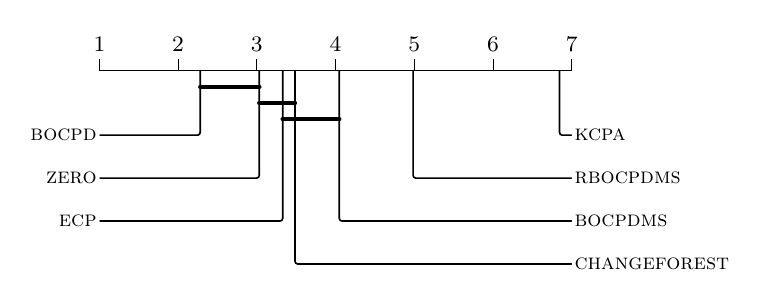
\begin{tikzpicture}
\begin{axis}[axis x line=center,%
axis y line=none,%
xmin=1,%
xmax=7,%
ymin=-5.5,%
ymax=0,%
clip=false,%
scale only axis,%
height=3cm,%
width=6cm,%
ticklabel style={
anchor=south,%
yshift=1.33*\pgfkeysvalueof{/pgfplots/major tick length},%
font=\footnotesize},%
every tick/.style={
yshift=.5*\pgfkeysvalueof{/pgfplots/major tick length}},%
xtick={1,...,7},%
axis line style={-},%
title style={
yshift=\baselineskip}]

\draw[semithick, rounded corners=1pt]
(axis cs:2.28125, 0) |- (axis cs: 1, -1.5)
node[font=\footnotesize, fill=white, inner xsep=1pt, outer xsep=0pt, anchor=east]
{\textsc{bocpd}};

\draw[semithick, rounded corners=1pt]
(axis cs:3.03125, 0) |- (axis cs: 1, -2.5)
node[font=\footnotesize, fill=white, inner xsep=1pt, outer xsep=0pt, anchor=east]
{\textsc{zero}};

\draw[semithick, rounded corners=1pt]
(axis cs:3.328125, 0) |- (axis cs: 1, -3.5)
node[font=\footnotesize, fill=white, inner xsep=1pt, outer xsep=0pt, anchor=east]
{\textsc{ecp}};

\draw[semithick, rounded corners=1pt]
(axis cs:3.484375, 0) |- (axis cs: 7, -4.5)
node[font=\footnotesize, fill=white, inner xsep=1pt, outer xsep=0pt, anchor=west]
{\textsc{changeforest}};

\draw[semithick, rounded corners=1pt]
(axis cs:4.046875, 0) |- (axis cs: 7, -3.5)
node[font=\footnotesize, fill=white, inner xsep=1pt, outer xsep=0pt, anchor=west]
{\textsc{bocpdms}};

\draw[semithick, rounded corners=1pt]
(axis cs:4.984375, 0) |- (axis cs: 7, -2.5)
node[font=\footnotesize, fill=white, inner xsep=1pt, outer xsep=0pt, anchor=west]
{\textsc{rbocpdms}};

\draw[semithick, rounded corners=1pt]
(axis cs:6.84375, 0) |- (axis cs: 7, -1.5)
node[font=\footnotesize, fill=white, inner xsep=1pt, outer xsep=0pt, anchor=west]
{\textsc{kcpa}};

\draw[ultra thick, line cap=round]
(axis cs:2.28125, -0.375) -- (axis cs:3.03125, -0.375);

\draw[ultra thick, line cap=round]
(axis cs:3.03125, -0.75) -- (axis cs:3.484375, -0.75);

\draw[ultra thick, line cap=round]
(axis cs:3.328125, -1.125) -- (axis cs:4.046875, -1.125);

\end{axis}
\end{tikzpicture}
\end{document}